\chapter{ПРОГРАМНИЙ МОДУЛЬ ВИЗНАЧЕННЯ МЕТРИК ЦІЛЬОВОЇ ПРОГРАМИ ДЛЯ ПІДВИЩЕННЯ ЕФЕКТИВНОСТІ ДОСЛІДЖЕННЯ ЇЇ ПОТЕНЦІЙНО-НЕБЕЗПЕЧНИХ ДЕФЕКТІВ}
\label{3section::doc}\label{3section:id1}

\section{Структурна схема алгоритму та основні функціональні елементи}
\label{3section:id2}
Підчас аналізу предметної області мною була запропонована структурна схема програмно-технічного комплексу виявлення залежностей між метриками інтегрованих властивостей програм.
\begin{figure} [h]
    \centering
    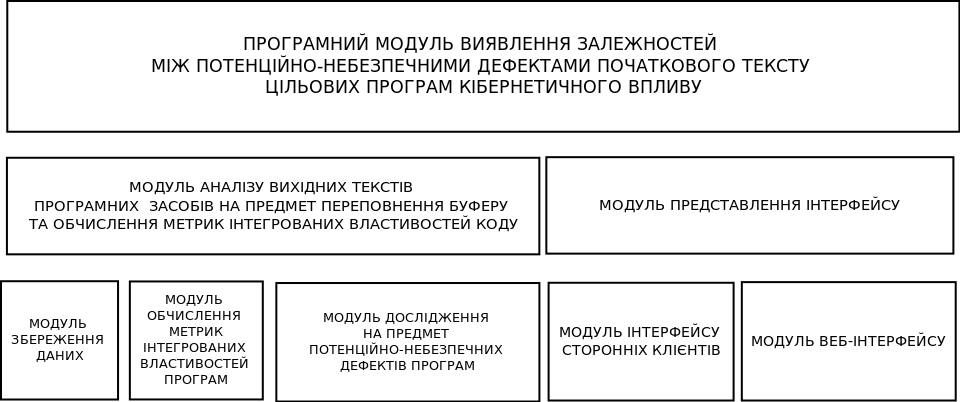
\includegraphics[width=16cm]{general_structure.png}
    \caption{Структурна схема модулю визначення метрик цільової програми}
    \label{fig:general_structure}
\end{figure}
(Рис \,\ref{fig:general_structure})

Модулі програмно-технічного комплексу:
\begin{enumerate}
 \item Модуль аналізу вихідних текстів програмних засобів на предмет переповнення буферу та обчислення метрик інтегрованих властивостей коду;
 \item Модуль представлення інтерфейсу.
\end{enumerate}

Модуль аналізу вихідних текстів програмних засобів включає в себе декілька підмодулів:
\begin{itemize}
 \item Модуль обчислення метрик інтегрованих властивостей програм;
 \item Модуль досліджнення на предмет потенційно-небезпечних дефектів програм;
 \item Модуль збереження даних.
\end{itemize}

В свою чергу, модуль представлення інтерфейсу містить 2 підмодулі:
\begin{itemize}
 \item Модуль веб-інтерфейсу
 \item Модуль інтерфейсу сторонніх клієнтів
\end{itemize}

В цілому програмний модуль реалізовано на базі {\itshape Google App Engine}  - платформі, що являє собою хмарний сервіс.

Зараз багато говорять про хмарні сервіси та хмарні обчислення. Економічну ефективність хмарних сервісів вже оцінив бізнес, а їх зручність – пересічний користувач. Часом можна зустріти компанію або користувачів, які активно працюють з хмарними сервісами, не підозрюючи про те, що вони знаходяться "на передньому краї" сучасних {\itshape ІТ}-технологій, а їх дії відповідають найновішим трендам {\itshape ІТ}-галузі.

Під хмарними обчисленнями розуміють інструменти, які доступні користувачу через інтернет або локальну мережу у вигляді веб-сервісу. Управляти такими інструментами можна лише за допомогою браузера. Таким чином можна отримати віддалений доступ до певних ресурсів (обчислювальних ресурсів, програм, даних) – хмарних сервісів. Основна перевага хмарних обчислень полягає в тому, що користувач чи клієнт сплачує лише за фактичне використання обчислювальних сервісів, а не за володіння ними. Наприклад, для компанії, яка лише починає працювати на ринку і для якої не потрібні потужні ресурси, але яка потенційно планує активно розширюватись, це особливо зручно. Купити готові програмні рішення та відповідне апаратне забезпечення (комп’ютери, сервера) буде доволі дорого на початку, а ось оплата лише за використані ресурси є доступною практично для всіх. Водночас при розширенні клієнтської бази та збільшенні необхідності щодо обчислювальних ресурсів компанії буде достатньо лише заявити про це своє бажання своєму постачальнику хмарних технологій та перейти на інший тарифний план. В результаті цього з мінімальними затратами часу і сил клієнт отримає ресурси, які відповідають його запитам у кожний конкретний момент часу.

Однією з перших компаній, яка запропонувала своїм клієнтам хмарний сервіс була компанія {\itshape Salesforce.com} – клієнтам {\itshape Salesforce.com} було запропоновано не купувати у компанії готові рішення (які були досить дорогими), а підписуватись на послуги {\itshape Salesforce.com}, отримуючи цілий ряд переваг. В результаті такого аутсорсингу інформаційних послуг, клієнти {\itshape Salesforce.com} отримували можливість використання продуктів {\itshape Salesforce.com}, встановлених на їх серверах, захист від збоїв, технічну підтримку.

{\itshape Salesforce.com} почала пропонувати свої рішення в 2000 році, а уже в 2005 році компанія {\itshape Amazon} вийшла на цей ринок із рішенням {\itshape \dq Amazon Web Services\dq}. Починаючи з 2006 року одним з найбільших представників ринку хмарних сервісів стала компанія Google з її продуктом {\itshape \dq Google Apps\dq}, а згодом і {\itshape Microsoft} з {\itshape \dq Azure Services Platform\dq}.

Хмарні обчислення найчастіше класифікують відповідно до їх змісту і призначення. Хмарні технології можна розділити на такі види

\begin{enumerate}
\item Програмне забезпечення як сервіс {\itshape (\dq Software as a Service\dq або \dq SaaS\dq)} – програмне забезпечення у вигляді сервісу, доступ до якого здійснюється через веб. Саме до цього виду можна віднести більшість хмарних сервісів для користувачів;
\item Інфрастуктура як сервіс {\itshape (\dq Infrastructure as a Service\dq або \dq IaaS\dq)} – надання платформи віртуалізації у форматі послуги;
\item Платформа як сервіс {\itshape (\dq Platform as a Service\dq або \dq PaaS\dq)} – надання платформи для розробки, тестування, розсортування і підтримки веб-додатків
\end{enumerate}

Види хмарних технологій {\itshape IaaS} та {\itshape PaaS} найчастіше використовуються розробниками для створення нових продуктів та {\itshape ІТ}-фахівцями, які працюють над вирішенням бізнес-задач.

Одним з перших і найпопулярніших хмарних інструментів є продукт {\itshape Amazon Web Services}, до складу якого увійшли засоби для збереження {\itshape (Simple Storage Service, SimpleDB)} и обробки {\itshape (EC2, EC2 MapReduce)}, а також послуги для організації хмарних мереж і хмарних додатків, наприклад, {\itshape Amazon Mechanical Turk (Mturk), Amazon Historical Pricing, Amazon Flexible Payments Service (FPS)} .

Компанія {\itshape Google} пропонує хмарне середовище {\itshape Google App Engine}, в якому можна запускати додатки, написані на мові {\itshape Python} із додатковою підтримкою фреймворків {\itshape Django, WebOb и PyYAML}, а також додатки на {\itshape Java}.

Ще одне рішення від {\itshape Google} – набір хмарних сервісів {\itshape Google Apps}, до складу якого входять електронна пошта {\itshape Gmail}, веб-календар {\itshape Google Calendar}, інструмент комунікації {\itshape Talk}, система роботи з документами {\itshape Google Docs} і сервіс для створення сайтів {\itshape Sites}. Всі ці сервіси інтегровані між собою і підтримують взаємодію за допомогою скриптів на {\itshape javascript}, які підтримуються для всіх клієнтів {\itshape Apps Premier} и {\itshape Education Edition}.

Хмарні сервіси від{\itshape  Microsoft} включають хмарну платформу {\itshape Windows Azure Platform} и набір хмарних сервісів {\itshape (.NET, SQL Azure, Live, SharePoint, Dynamics CRM)}. {\itshape Windows Azure} представляє собою платформу і інфраструктуру для запуску {\itshape Windows}-додатків в хмарному середовищі.

Не дивлячись на цілий ряд переваг хмарних сервісів (доступність, економічність і ефективність, гнучкість) існують й проблеми для їх розповсюдження і використання. Вочевидь, хмарні сервіси вимагають постійного інтернет-з’єднання, що є не завжди доступним, особливо у регіонах. Потенційні клієнти часто не довіряють хмарним сервісам через можливі проблеми з безпекою даних. Окрім того, розповсюдження хмарних сервісів вимагає наявності у країні потужних центрів обробки даних. І головне – не всі інструменти або програми можуть бути доступними у віддаленому режимі.


\subsubsection{Модуль аналізу вихідних текстів програмних засобів}
\label{module_analize}
Даний модуль реалізує аналіз метричних характеристик досліджуваних програм та потенційно-небезпечних дефектів реакції програм, та на основі цих даних робить кількісну оцінку вразливих участків коду. Дані характеристики зберігаються в {\itshape Google Cloud SQL} за допомогою {\it NDB API}.

{\itshape Google Cloud SQL}-це служба, яка дозволяє створювати, настроювати і використовувати реляційні бази даних, які розміщені в {\itshape Google Cloud}. Це повністю керований сервіс, що веде, керує і розпоряджається вашими базами даних, дозволяючи вам зосередитися на ваших додатків і послуг.

Інтерфейс {\itshape NDB} зберігає дані об'єкти, відомі як сутності.
{\itshape NDB} можете згрупувати кілька операцій в одну операцію. Транзакції не можуть досягти успіху, якщо хоча б одна операція в транзакції не завершується успішно або якщо який-небудь збій операції. Це особливо корисно для розподілених і веб-додатків, де декілька користувачів можуть мати доступ до або маніпулювання даними одночасно.

{\itshape NDB} використовує {\itshape Memcache} в якості кеша служби для "гарячих точок" у даних. Якщо додаток зчитує деякі дані часто, {\itshape NDB} можете читати їх швидко з кешу.

Як було вище сказано ( підрозділ \ref{2section:id13}) метрики вихідного тексту в сукупності зі знайденими вразливостями підставляються в формулу \eqref{eq:my_equation}, і обчислюється потенціал вихідного коду, який буде використаний для обчислення ймовірності використання вразливостей даного модулю.
В БД зберігаються всі потенціали вихідних текстів, які містять потенційні вразливості разом з ймовірностями, які вираховуються за допомогою лінійної екстраполяції елементів, розміщених в БД. Ці ймовірності являються експериментальними і в процесі дослідження і роботи спеціалістів над певними вихідними текстами проекту можуть бути змінені вручну, для збільшення точності оцінювання.
Екстраполювання виконується за допомогою бібліотеки {\it NumPy}.

{\it NumPy} - бібліотека мови {\it Python} для роботи з гомогенними багатовимірними масивами даних, які індексуються додатніми цілими числами. Гомогенність даних дозволяє значно оптимізувати роботу в порівнянні з стандартними списками мови.
Основний тип даних відповідно - array.
На базі {\it NumPy} написано майже усе науково-технічне програмне забеспечення мовою {\it Python}, зокрема
українське ПЗ {\it OpenOpt} (чисельна оптимізація, автоматичне диференціювання, розв’язування систем рівнянь)
{\it SciPy} (інтеграція, інтерполяція, статистика і т.і.)
науково-інженерні {\it Python}-дистрибутиви {\it PythonXY, SAGE} (вільні аналоги до {\it MATLAB, Maple, MatCad, Mathematica} і т.і.)

Оскільки {\it Python} - інтерпретована мова, математичні алгоритми, часто працюють в ньому набагато повільніше ніж у компільованих мовах, таких як {\it C} або навіть {\it Java}. {\it NumPy} намагається вирішити цю проблему для великої кількості обчислювальних алгоритмів забезпечуючи підтримку багатовимірних масивів і безліч функцій і операторів для роботи з ними. Таким чином будь-який алгоритм який може бути виражений в основному як послідовність операцій над масивами і матрицями працює також швидко як еквівалентний код написаний на {\it C}.

{\it NumPy} можна розглядати як вільну альтернативу {\it MATLAB}, оскільки мова програмування {\it MATLAB} зовні нагадує {\it NumPy}: обидві вони інтерпретовані, і обидві дозволяють користувачам писати швидкі програми поки більшість операцій проводяться над масивами або матрицями, а не над скалярами. Перевага {\it MATLAB} у великій кількості доступних додаткових тулбоксів, включаючи такі як пакет {\it Simulink}. Основні пакети, що доповнюють {\it NumPy}, це: {\it SciPy} - бібліотека, що додає більше {\it MATLAB}-подібної функціональності; {\it Matplotlib} - пакет для створення графіки в стилі {\it MATLAB}. Внутрішньо як {\it MATLAB}, так і {\it NumPy} базується на бібліотеці {\it LAPACK}, призначеної для вирішення основних задач лінійної алгебри.

\subsubsection{Модуль обчислення метрик інтегрованих властивостей програм}
\label{module_metrix_calculations}
Даний модуль реалізує аналіз вихідного коду програмного забезпечення - а саме обчислення метрик інтегрованих властивостей програмного коду - метрики Холстеда, Маккейба, Джилба, за допомогою побудови абстрактного синтаксичного дерева програмного коду з наступним його аналізом.

Абстрактні синтаксичні дерева зазвичай використовуються при компіляції,
коли для нас важлива лише функціональна складова даних, маючи яку ми зможемо згенерувати байткод програми, який буде виконуваті дії, записані у вихідному
коді. Основне завдання даної моделі — збереження інформації у такій структурі,
яка дозволить легко  аналізувати вихідний код, а також генерувати його. Це  передбачає збереження якомога більшої кількості  інформації у моделі.

\subsubsection{Модуль досліджнення на предмет потенційно-небезпечних дефектів програм}
\label{module_vulnurabilities_search}
Даний модуль реалізує аналіз вихідного коду програмного забезпечення з використанням бібліотеки {\itshape Flawfinder}.
Ця бібліотека реалізує статичний сканер вихідних текстів програм, написаних на {\itshape С/С++}. Виконує пошук функцій, які найчастіше використовуються некоректно, присвоює їм коефіцієнти ризику (спираючись на таку інформацію, як передані параметри) і складає список потенційно вразливих місць, впорядковуючи їх за ступенем ризику.

\subsubsection{Модуль збереження даних}
\label{module_data_storing}
Даний модуль містить опис моделей представлення та збереження даних, отриманих в процесі аналізу вихідних текстів програм.
Головними сутностями данної моделі є проект, вихідний текст, метрика та вразливість.

%\inputminted[linenos,fontsize=\scriptsize]{python}{script.py}
%\newminted{python}{gobble=4,linenos,fontsize=\scriptsize}

\lstinputlisting [firstline=5] %,lastline=20]
{../src/app/models.py}

\subsubsection{Модуль представлення інтерфейсу}
\label{module_interface}
Модуль представлення інтерфейсу являє собою реалізацію Веб-інтерфейсу та інтерфейсу сторонніх клієнтів. Він реалізований на базі веб-фреймворків {\itshape webapp2} та {\itshape endpoints}.

\subsubsection{Модуль веб-інтерфейсу}
\label{module_web_interface}
Як було сказано вище, модуль веб-інтерфейсу реалізований з використанням фреймворку  {\itshape webapp2}. Основними його функціями являються:
\begin{enumerate}
\item Завантаження вихідних текстів проекту для наступного аналізу
\item Проведення аналізу проекту за допомогою вищенаведених модулів
\item Представлення даних аналізу в графічному та табличному вигляді
\item Корекція результатів аналізу
\end{enumerate}

\begin{figure}[h]
    \centering
    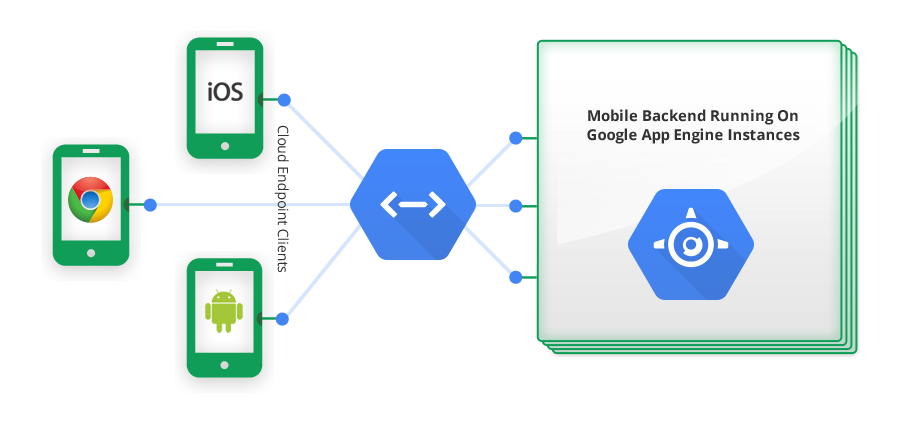
\includegraphics[width=18cm, height=10cm]{endpoints.png}
    \caption{приклад використання {\itshape endpoints}}
    \label{fig:endpoints_image}
\end{figure}

\subsubsection{Модуль інтерфейсу сторонніх клієнтів}
\label{module_endpoints}
Модуль інтерфейсу сторонніх клієнтів реалізовано з використанням бібліотеки {\itshape endpoints}, являє собою засіб забезпечення взаємодії між інтерфейсним модулем та сторонніми розробками, що дозволяє злегкістю розробляти програмні додатки на різних мовах програмування.


{\itshape Google Cloud Endpoints} складається з інструментів, бібліотек і можливостей, які дозволяють генерувати інтерфейси і клієнтські бібліотеки з {\itshape  App Engine}, їх також називають {\itshape API backend}, для спрощення доступу клієнтів до даних з інших додатків. {\itshape Endpoints} полегшють створення веб-серверної частини для веб-клієнтів і мобільних клієнтів, таких як {\itshape Android} або {\itshape Apple iOS} (Рис.\,\ref{fig:endpoints_image}).

\pagebreak

\section{Інтерфейс користувача}
\label{3section:id3}
Інтерфейс користувача являє собою Веб-додаток, що дозволяє завантажувати вихідні тексти досліджуваних проектів, та представляти їхні метрики та потенційні вразливості за допомогою діаграм {\itshape Google Charts}.

{\itshape Google Charts} забезпечує ідеальний спосіб візуалізації даних на веб-сайті. Бібліотека надає велику кількість готових до використання типів діаграм.

Найбільш поширений спосіб використання {\itshape Google Charts} з допомогою скриптів {\itshape JavaScript}, які можна вбудовувати в web-сторінки. Спочатку відбувається завантаження {\itshape Google Charts} бібліотек, перелік даних для побудови діаграми, проводиться вибір параметрів для настройки діаграми, і, нарешті, створення об'єктів {\itshape chart} з {\itshape id}, який ви вибираєте. Потім, пізніше у веб-сторінки, можна створити тег {\itshape <div>} з допомогою цього ідентифікатора для відображення {\itshape Google Chart}.

Це все, що потрібно для початку роботи.

Графіки представлені у вигляді класів {\itshape JavaScript}, і {\itshape Google Charts} дає багато типів діаграм, які можна використовувати. Зовнішній вигляд за замовчуванням, зазвичай реалізує все, що потрібно в більшості випадків, і завжди існує можливість  налаштування діаграми, щоб підігнати зовнішній вигляд до веб-сайту. {\itshape Google Charts} є інтерактивними та дозволяють задавати реакцію на події від користувача, що дозволяє підключати їх до створення складних інформаційних панелей, інтегрованих з вашої веб-сторінці. Діаграми будуються з використанням {\itshape HTML5/SVG} технології для забезпечення сумісності з різними браузерами (у тому числі {\itshape VML} для більш старих версій {\itshape IE}) і крос-платформену переносимість {\itshape iPad і iPhone і Android}.

\begin{figure}[h]
    \centering
    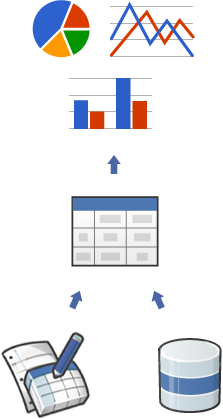
\includegraphics[width=8cm]{visualization_intro.png}
    \caption{приклад використання {\itshape Google Charts}}
    \label{fig:googlecharts_image}
\end{figure}

Всі типи діаграм, які заповнюються даними, використовуючи клас {\itshape DataTable}, що дозволяє легко перемикатися між типами діаграм, щоб дозволить легко підібрати найбільш підходящий тип діаграми для представлення данних. {\itshape DataTable} надає методи для сортування, редагування та фільтрації даних, і можуть бути заповнені безпосередньо з веб-сторінки, бази даних, або будь-яких джерел даних, що підтримують інструменти {\itshape Charts Datasource} протоколу. (Цей протокол включає в себе {\itshape SQL}-подібний мову запитів і реалізується за допомогою електронних таблиць, {\itshape Google} зведених таблиць, а також сторонні постачальники даних, таких як {\itshape SalesForce}.

\begin{figure}[h]
    \centering
    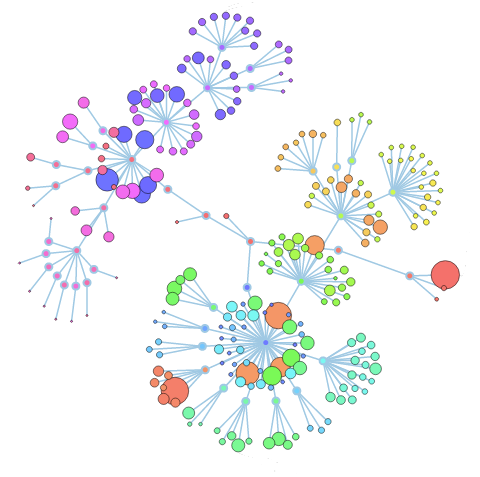
\includegraphics[width=16cm]{code_flower_demo.png}
    \caption{приклад дерева, побудованого з допомогою {\it CodeFlower}}
    \label{fig:codeflower_demo_image}
\end{figure}

Існує також можливість реалізації власного протоколу для створенння свого провайдеру даних для своїх додатків (Рис.\,\ref{fig:googlecharts_image}).

Окрім бібліотеки {\itshape Google Charts}, в модулі інтерфейсу користувача використано бібліотеку {\itshape CodeFlower}.

{\itshape CodeFlower}, реалізована на базі {\itshape JavaScript}-фреймворку {\itshape d3.js}, вона показує репозиторії вихідних кодів з використанням інтерактивного дерева. Кожний вузол являє собою файл, з радіусом пропорційно значенні певної характеристики заданого вузла. Вся візуалізація виконується на стороні клієнта, в {\itshape JavaScript}. При наведенні курсору на будь-який вузол відображається назва файлу та його властивості (Рис.\,\ref{fig:codeflower_demo_image}).

Також для представлення вихідних текстів програм для загального огляду та аналізу було використано бібліотеку {\it CodeMirror}.

{\it CodeMirror} - це потужна бібліотека для підсвічування синтаксису близько сорока з гаком мов програмування і розмітки. Головною відмінністю від досить відомого {\it Syntax Highlighter} є реалізація динамічного просунутого підсвічування коду буквально на ходу, як це приміром реалізовано в настільних додатках типу {\it Geany} або {\it Notepad++}. Крім усього іншого присутня налаштування клавіш швидкого доступу, показ ключових слів по {\it Ctrl+Space}, виділення поточної рядки (де зупинився курсор мишки), напівавтоматична розстановка відступів і багато багато іншого.

{\it CodeMirror} є внутрішньо-браузерним {\it javascript}-компонентом, який був розроблений {\it Marijn Haverbeke}. {\it CodeMirror} сумісний з {\it Firefox} 3 або вище, {\it Google Chrome, Safari} 5.2 або вище, {\it Opera} 9 або вище, а також {\it Internet Explorer} 8 або вище в стандартному режимі.

\begin{figure}[h]
    \centering
    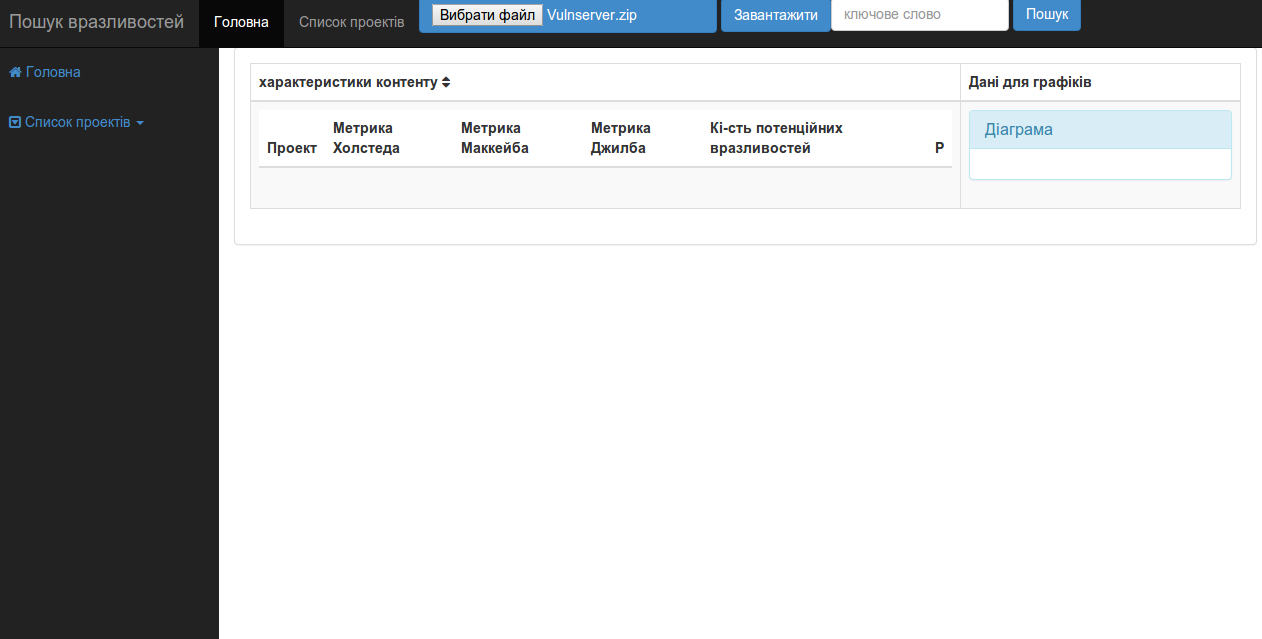
\includegraphics[width=17cm]{prj_main.png}
    \caption{головна сторінка}
    \label{fig:prj_main_image}
\end{figure}

Загалом, інтерфейс користувача є доволі простим та інтуєтивним (Рис.\,\ref{fig:prj_main_image}).

Для підготовки проекту до аналізу необхідно зробитти його зжаття та архівування в формат {\itshape zip}.
Після вивантаження зжатого архіву на сервер відбувається його розархівування з наступним аналізом всіх файлів, які він містить на предмет вразливостей та обчислення вищенаведених метрик його коду, з занесенням в БД відповідних результатів аналізу.

\begin{figure}[h]
    \centering
    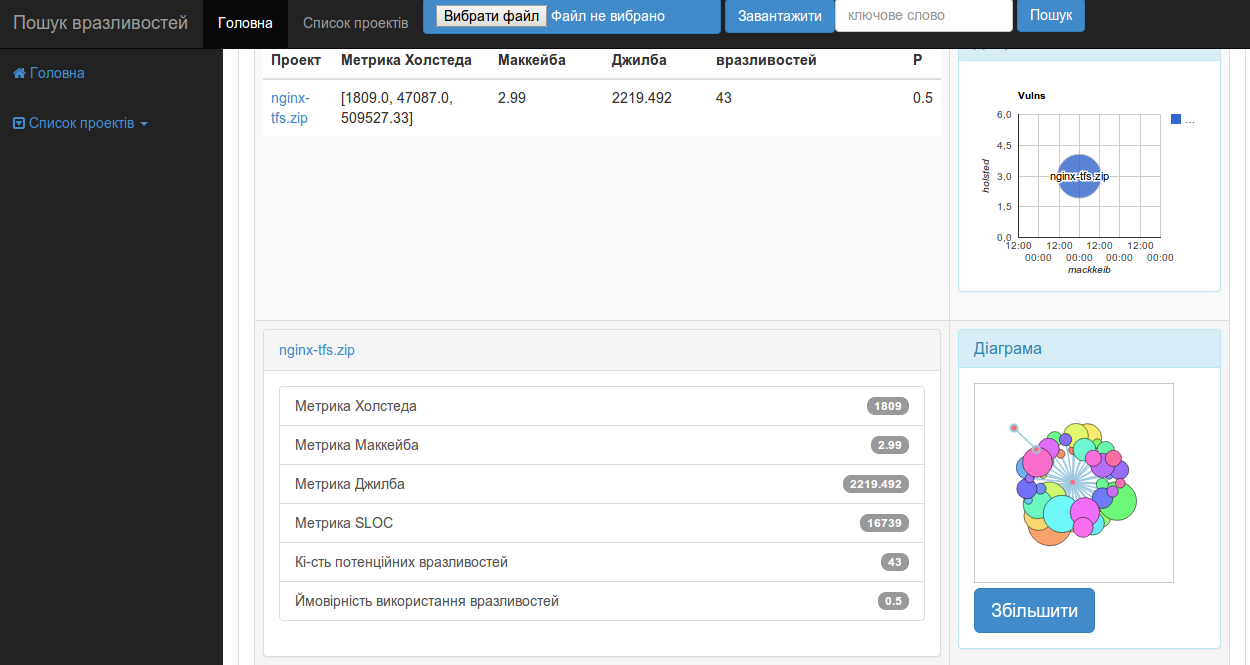
\includegraphics[width=17cm]{prj_project.png}
    \caption{властивості проекту}
    \label{fig:prj_project_image}
\end{figure}

Після даної операції існує можливість переглянути його властивості, зробити висновок щодо організації подальшого досліджнення цільових програм для реалізації кібернетичного впливу.

На сторінці списку завантажених(проаналізованих) проектів виводиться список проктів, елементами якого є пара - таблиця та відповідна діаграма, яка відображає властивості проекту.

Окрім цього можна також скористатись навігацією по вихідним текстам проекту, де також відображається інформація про метрики коду та кількість потенційних вразливостей для кожного файлу проекту (Рис.\,\ref{fig:prj_project_image}).

\pagebreak[4]

\section{Керівництво щодо розгортання та експлуатації}
\label{3section:id4}

Для встановлення та налаштування роботи програмного модулю необхідно встановити наступні складові:
\begin{enumerate}
\item встановити інтерпретатор {\it Python 2.7};
\item встановити менеджер пакетів {\it Python - PIP};
\item завантажити з офіційного сайту та встановити пакет інструментальних засобів {\it Google App Engine SDK};
\item за допомогою менеджеру пакетів встановити бібліотеку лінійної алгебри {\it NumPy};
\item завантажити {\it Google App Engine Launcher} - програмний засіб управління {\it Google App Engine};
\item запустити програмний модуль за допомогою {\it Google App Engine Launcher}.
\item за допомогою браузера здійснити доступ до веб-сервісі, по налаштованому порту.
\end{enumerate}

Розглянемо дещо детальніше даний процес для операційної системи Linux:

встановимо {\it Python}
\begin{lstlisting}[language=bash] 
$ sudo apt-get install python27
\end{lstlisting}

встановимо пекетний менеджер {\it Python}
\begin{lstlisting}[language=bash] 
$ sudo apt-get install python-pip27
\end{lstlisting}

встановимо {\it Google App Engine SDK}
\begin{lstlisting}[language=bash] 
$ c d /tmp
$ wget http://googleappengine.googlecode.com/files/google_appengine_1.8.9.zip
$ unzip google_appengine_1.8.9.zip
$ c d google_appengine
$ sudo python setup.py build install
\end{lstlisting}

за допомогою менеджеру пакетів встановимо бібліотеку лінійної алгебри {\it NumPy}
\begin{lstlisting}[language=bash] 
$ sudo pip install numpy
\end{lstlisting}

завантажимо {\it Google App Engine Launcher} - програмний засіб управління {\it Google App Engine}
\begin{lstlisting}[language=bash] 
$ c d /opt/
$ svn checkout http://google-appengine-wx-launcher.googlecode.com/svn/trunk/ google-appengine-wx-launcher-read-only
$ c d google-appengine-wx-launcher-read-only
$ python GoogleAppEngineLauncher.py
\end{lstlisting}

запустимо програмний модуль за допомогою {\it Google App Engine Launcher}
\begin{lstlisting}[language=bash] 
$ dev_appserver.py <path to project.module>
\end{lstlisting}

\pagebreak

\section*{Висновки}
\addcontentsline{toc}{section}{Висновки}
Отже, підводячи підсумок практичної реалізації можна зазначити, що мета оцінки та програмного коду для ефективної організації аналізу проектів на предмет можливості використання їх потенційно-небезпечних вразливостей досягнута. Вищеперераховані програмні методи можуть бути використані в подальшому в мережах спеціального призначення.
